\documentclass{article}
\usepackage[utf8]{inputenc}
\usepackage{graphicx}

\title{Practicatalf 2}
\author{Jose Antonio Guardeño Algar}
\date{October 2022}

\begin{document}

\maketitle

\section{Activities}
\subsection{1}
\begin{tabular}{| c | c | c |}
\hline
\delta(q, σ) & a & b \\ \hline
q_0 & q_1 & q_3 \\
q_1 & q_3 & q_3\\
q_3 & q_3 & q_3\\ \hline
\end{tabular}
\newline
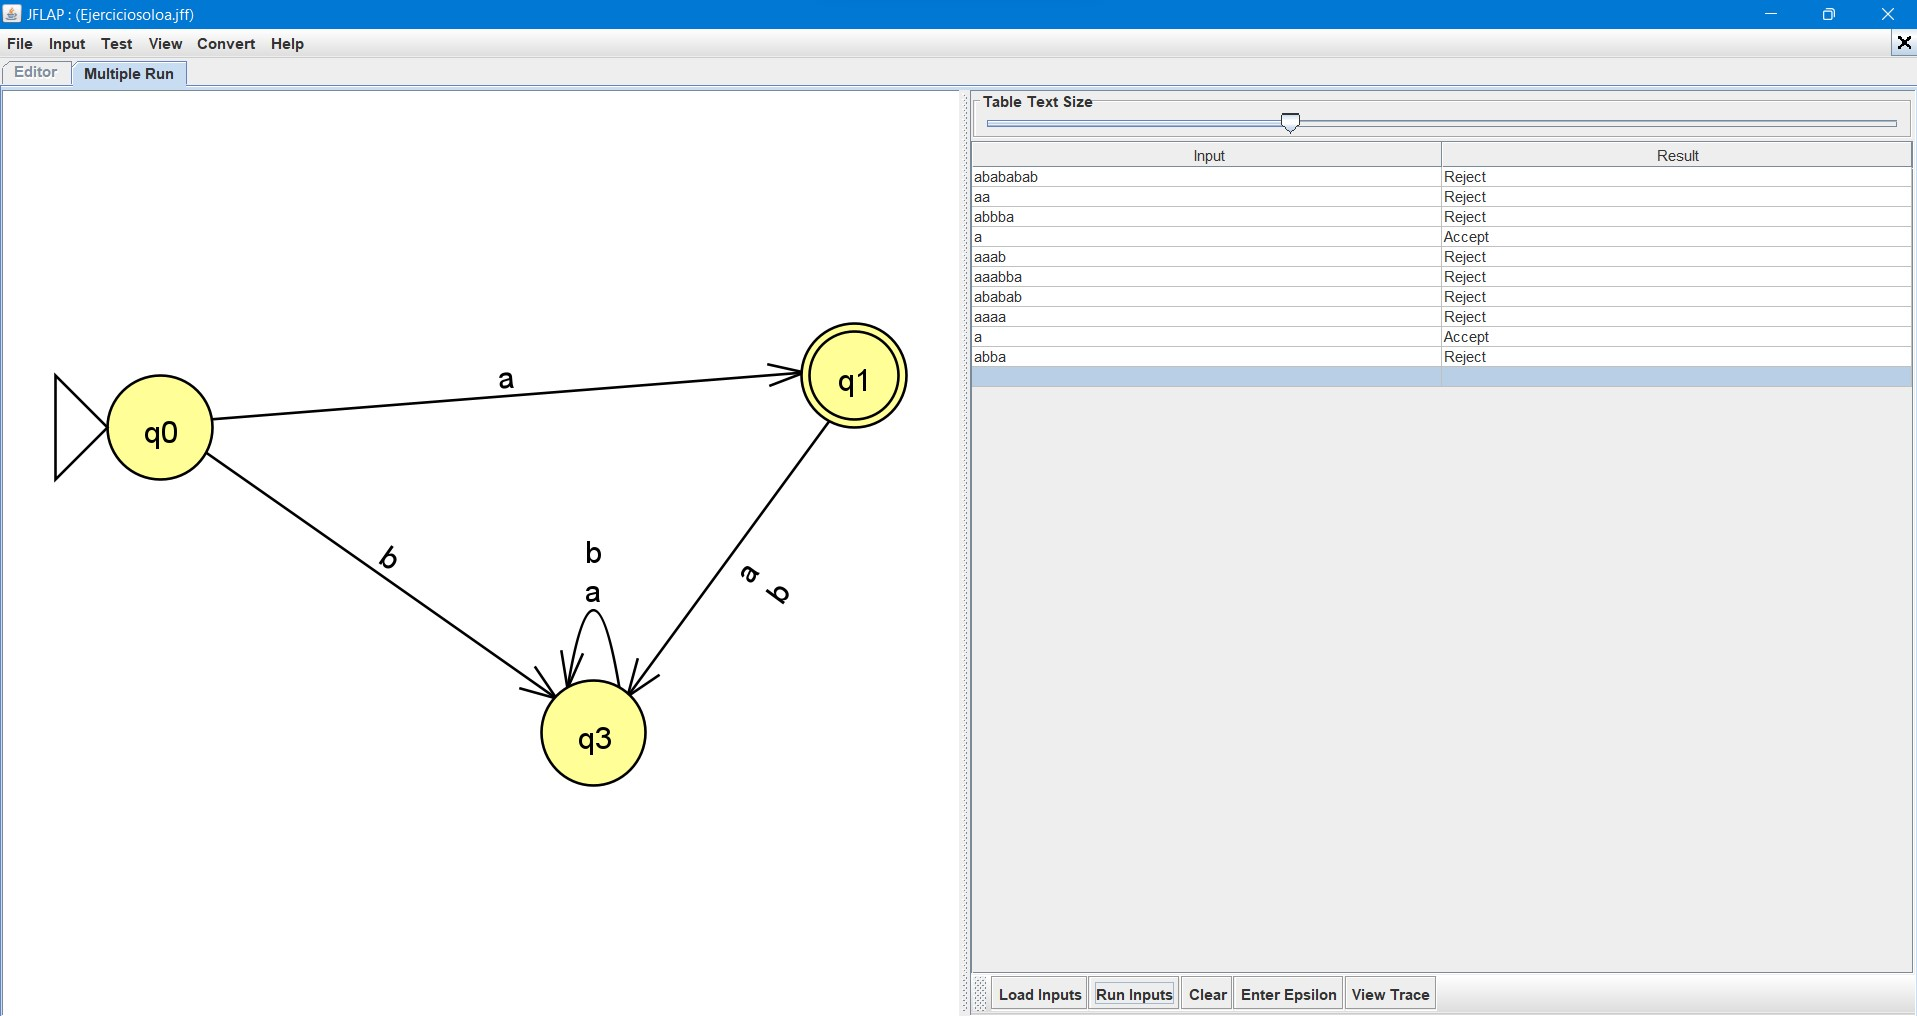
\includegraphics[width=15cm]{soloajpg.jpg}
\subsection{2}
\begin{verbatim}
    {
    "name" : "soloa",
    "representation" : {
      "K" : ["q0", "q1","q3"],
      "A" : ["a", "b"],
      "s" : "q0",
      "F" : ["q1"],
      "t" : [["q0", "a", "q1"],
             ["q0", "b", "q3"],
             ["q1", "a", "q3"],
             ["q1", "b", "q3"],
             ["q3", "a", "q3"],
             ["q3", "b", "q3"]]
      }
  },
\end{verbatim}
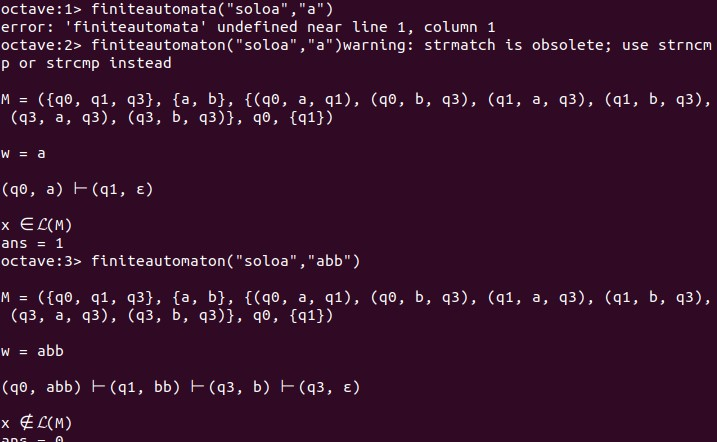
\includegraphics[width=15cm]{octavefin13.jpg}
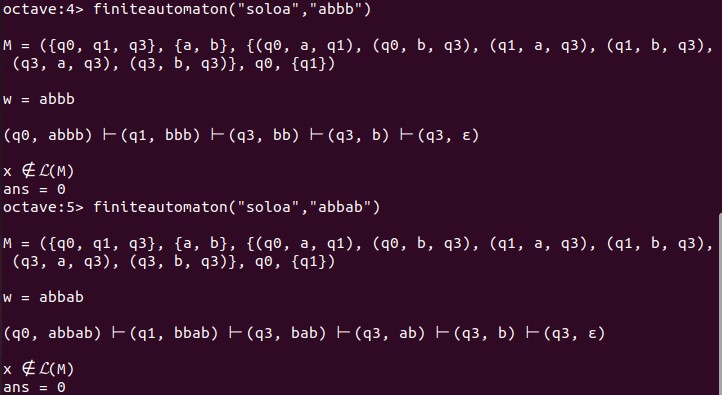
\includegraphics[width=15cm]{octav32.jpg}
\end{document}
